
\section{Algebraic preliminaries}

Fix a commutative ring with unit $R$. 
We work over the symmetric monoidal category $(\Ch, \otimes, R)$ of chain complexes of $R$-modules.
As usual, we regard the set of $R$-linear maps $\Hom(C, C^\prime)$ between chain complexes as a chain complex.
The $i\th$ suspension functor $s^i \colon \Ch \to \Ch$ is defined on objects by $(s^{i}M)_n= M_{n-i}$.

A \textit{coassociative counital coalgebra} $C=(C, \partial, \Delta, \varepsilon)$ is the data of an object $(C, \partial) \in \Ch$ equipped with maps $\Delta: C \to C \otimes C$ and $\varepsilon: C\to R$ in $\Ch$ satisfying the usual coassociativity and counitality equations, respectively. 

This notion is equivalent to that of a comonoid in the $(\Ch, \otimes, R)$. Denote by $\coAlg$ the category of coassociative counital coalgebra with morphisms being maps that preserve the structure. 

We notice that $(\coAlg, \otimes, R)$ is symmetric monoidal with structure maps:
\begin{center}
\begin{tikzcd}
C \otimes C^\prime \arrow[r, "\Delta \otimes \Delta^\prime"] &
(C \otimes C) \otimes (C^\prime \otimes C^\prime) \arrow[r, "(23)"] &
(C \otimes C^\prime) \otimes (C \otimes C^\prime),
\end{tikzcd} \par
\begin{tikzcd}
C \otimes C^\prime \arrow[r, "\varepsilon \otimes \varepsilon^\prime"] &
R \otimes R \arrow[r, "\cong"] &
R.
\end{tikzcd}
\end{center}

We will denote the category of monoids on a symmetric monoidal category $\C$ by $\Mon_{\C}$.\footnote{Monoids in $\Ch$ and $\coAlg$ are sometimes referred to as differential graded associative unital algebras and bialgebras respectively, but we avoid this terminology.}




\subsection{The cobar construction}

Let $C$ be a coassociative counital coalgebra.
A \textit{coaugmentation} is a morphism $\nu \colon R \to C$ in $\coAlg$.
Denote by $\coAlg^*$ the category of \textit{coaugmented coassociative counital coalgebras} with morphisms being structure preserving chain maps.

We recall the definition of the \textit{cobar} functor 
\begin{equation*}
\cobar \colon \coAlg^* \to \Mon_{\Ch}.
\end{equation*}

Let  $(C, \partial, \Delta, \varepsilon, \nu)  \in \coAlg^*$ where $\nu: R \to C$ is the coaugmentation. Define
$$\mathbf{\Omega}(C, \partial, \Delta, \varepsilon, \nu) := ( T(s^{-1}  \overline{C} ), D, \mu) \in \Mon_{\Ch}$$ where 
\begin{itemize}
\item $\overline{C}=\text{coker}(\nu: R \to C)$
\item $T(s^{-1} \overline{C})= R \oplus \overline{C} \oplus (\overline{C}  \otimes \overline{C} ) \oplus ( \overline{C} \otimes \overline{C} \otimes \overline{C} ) \oplus\cdots $
\item $\mu: T(s^{-1}  \overline{C} )^{\otimes 2} \to T(s^{-1}  \overline{C} ) $ is the free associative unital product given by concatenation of monomials
\item $D: T(s^{-1}  \overline{C} ) \to T(s^{-1}  \overline{C} )$ is the derivation of degree $-1$ determined by extending the linear map $$- s^{-1} \circ \partial \circ s^{+1} + (s^{-1} \otimes s^{-1}) \circ \Delta \circ s^{+1}: s^{-1}\overline{C} \to s^{-1}\overline{C} \oplus (s^{-1}\overline{C} \otimes s^{-1}\overline{C}) \hookrightarrow T(s^{-1}C)$$ as a derivation.
\end{itemize}

The coassociativity of $\Delta$, the compatibility of $\partial$ and $\Delta$, and the fact that $\partial^2 =0$ together imply that $D^2=0$. This construction is clearly functorial with respect to maps in $\coAlg^*$. We will denote $\mathbf{\Omega} (C, \partial, \Delta, \varepsilon, \nu)$ simply by $\mathbf{\Omega}(C)$. 

In this article we are mostly concerned with \textit{connected} coalgebras, namely $C \in \coAlg^*$ which are non-negatively graded and the coaugmentation $\nu: R \to C$ induces an isomorphism of coalgebras $R \cong C_0$. We denote by $\coAlg^0$ the full subcategory of $\coAlg^*$ consisting of connected coalgebras. If $C \in \coAlg^0$, then $\mathbf{\Omega}(C)$ is concentrated on non-negative degrees. 

The cobar construction was originally applied by Adams' to the coalgebra of normalized chains on a $1$-reduced simplicial set to obtain a model for the chains on the based loop space \cite{Adams}. The cobar construction as a model for the based loop space was furthered studied in \cite{Baues} and more recently, in the non-simply connected setting in \cite{Hess-Tonks}, \cite{Rivera-Zeinalian}.


---
Discuss the localized version of the cobar construction. ---
%\section{The prop $\M$}

\subsection{Operads and props} \label{s:operads and props}

Let $(\C, \otimes, \mathbb{1})$ be either the category $(\Ch, \otimes, R)$ of dg $R$-modules or the category $(\coAlg_R, \otimes, \mathbb{1})$ of coassociative counital dg-coalgebras.
Both of these categories are closed symmetric monoidal.
Given objects $C, C^\prime \in \C$ we denote the dg $R$-module of $R$-linear maps between them as $\Hom(C, C^\prime)$. 

Recall that a group $G$ can be thought of as a category with a single object and only invertible morphisms. From this viewpoint, a left $G$-module (resp. right $G$-module or $G$-bimodule) is the same as a functor from $G$ (resp. $G^\op$ or $G \times G^\op$) to $\C$.

Let $\S$ be the category whose objects are the natural numbers and whose set of morphisms between $m$ and $n$ is empty if $m \neq n$ and is otherwise the symmetric group $\S_n$.
A \textit{left $\S$-module} (resp. right $\S$-module or $\S$-bimodule) is a covariant functor from $\S$ (resp. $\S^\op$ or $\S \times \S^\op$) to $\C$.
In this paper we prioritize left module structures over their right counterparts. As usual, taking inverses makes both perspectives equivalent.

The homomorphism $\S_n \to \S_n \times \S_1$ induces a forgetful functor $U$ from the category of $\S$-bimodules to that of $\S$-modules.

Given an object $C$ in $\C$ define:
\begin{align*}
\End^C(r) &= \Hom(C, C^{\otimes r}),
&\End^C_C(r, s) &= \Hom(C^{\otimes r}, C^{\otimes s}),
\end{align*}
with their natural structures of $\S$-module and $\S$-bimodule respectively.
The forgetful functor $U$ sends $\End^C_C$ to $\End^C$.

\textit{Operads} and \textit{props} are respectively $\S$-modules and \mbox{$\S$-bimodules} enriched with certain composition structures.
These are best understood by abstracting the composition structure naturally present in the $\S$-module $\End^C$, naturally an operad, and the $\S$-bimodule $\End^C_C$, naturally a prop.

Succinctly, an operad $\mathcal O$ is an $\S$-module together with a collection of $R$-linear maps
\begin{equation*}
\mathcal O(r) \otimes \mathcal O(s) \to \mathcal O(r+s-1)
\end{equation*}
satisfying suitable associativity, equivariance and unitality conditions.
A prop $\mathcal P$ is an $\S$-bimodule together with two types of compositions; horizontal
\begin{equation*}
\mathcal P(r_1, s_1) \otimes \mathcal P(r_2, s_2) \to \mathcal P(r_1 + r_2, s_1 + s_2)
\end{equation*}
and vertical
\begin{equation*}
\mathcal P(r,s) \otimes \mathcal P(s, t) \to \mathcal P(r, t)
\end{equation*}
satisfying their own versions of associativity, equivariance and unitality.
For a complete presentation of these concepts we refer to Definition 11 and 54 of \cite{Markl08}.

We remark that the compositional structure of a prop $\mathcal P$ restricts to operad structures on $U(\mathcal P)$.

An $E_\infty$-\textit{operad} is an operad whose underlying $\S$-module $M$ is such that $M(r)$ is free as a $\Z[\S_r]$-module and its homology is that of a point for every $r \geq 0$.

Following \cite{Getzler1994operads, Moerdijk1999monads} we refer to operads and props over the category $\coAlg$ as \textit{Hopf} operads and props.

\textit{Morphisms} of operads and props are those preserving all the structure.

Consider an object $C$ of $\C$, an operad $\mathcal O$ and a prop $\mathcal P$.
An $\mathcal O$-\textit{coalgebra} structure on $C$ is an operad morphism $\mathcal O \to \End^C$, and a $\mathcal P$-\textit{bialgebra} structure on $C$ is a prop morphism $\mathcal P \to \End_C^C$.

\subsection{The prop $\M$}

As described for example in \cite{Markl08, Fresse2010props}, the \textbf{free prop} $F(M)$ generated by a \mbox{$\S$-bimodule} $M$ is constructed using open directed graphs with no directed loops that are enriched with a labeling described next. We think of each directed edge as built from two compatibly directed half-edges. For each vertex $v$ of a directed graph $G$, we have the sets $in(v)$ and $out(v)$ of half-edges that are respectively incoming to and outgoing from $v$. Half-edges that do not belong to $in(v)$ or $out(v)$ for any $v$ are divided into the disjoint sets $in(G)$ and $out(G)$ of incoming and outgoing external half-edges. For any positive integer $n$, let $\overline{n} = \{1,\dots,n\}$ and $\overline{0} = \emptyset$. For any finite set $S$, denote the cardinality of $S$ by $|S|$. The labeling is given by bijections  
\begin{equation*}
\overline{|in(G)|} \to in(G), \qquad
\overline{|out(G)|} \to out(G),
\end{equation*}
and
\begin{equation*}
\overline{|in(v)|}\to in(v), \qquad
\overline{|out(v)|}\to out(v),
\end{equation*}
for every vertex $v$.
We refer to the isomorphism classes of such labeled directed graphs with no directed loops as $(n,m)$\textbf{-graphs} denoting the set of these by $\G(m,n)$.
We use graphs immersed in the plane to represent elements in $\G(m,n)$, please see Figure \ref{f:immersion}.
We consider the right action of $\S_n$ and the left action of $\S_m$ on a $(n,m)$-graph given respectively by permuting the labels of $in(G)$ and $out(G)$. This action defines the $\S$-bimodule structure on the free prop
\begin{equation} \label{e:free prop}
F(M)(m,n) \ = \bigoplus_{\Gamma \in \G(m,n)} \bigotimes_{v \in Vert(\Gamma)} out(v) \otimes_{\S_q} M(p, q) \otimes_{\S_p} in(v),
\end{equation}
where we simplified the notation writing $p$ and $q$ for $\overline{|in(v)|}$ and $\overline{|out(v)|}$ respectively. The composition structure is defined by (relabeled) grafting and disjoint union.

\input{immersion}

Let us consider the free prop $F(N)$ generated by the $\S$-bimodule $N$ whose only non-zero chain complexes are concentrated in degree $0$ and are give by
\begin{equation*}
N(1, 0)_0 = \Z\{\varepsilon\}, \qquad
N(1, 2)_0 = \Z[\S_2]\{\Delta\}.
\end{equation*}
Define $\A$ as the quotient of $F(N)$ by the prop ideal generated by the relations
\begin{equation*}
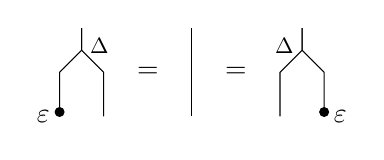
\begin{tikzpicture}[scale=.28]
\draw (-4,0)--(-4,2)--(-5,3)--(-5,4);
\draw (-6,0)--(-6,2)--(-5,3)--(-5,4);
\node [scale=.8] at (-4.2,3.2) {$\Delta$};
\draw [fill] (-6,.2) circle [radius=.2];
\node [left] at (-6,0) {$\varepsilon$};

\node at (-2,2) {=};
\draw (0,0)--(0,4);
\node at (2,2) {=};

\draw (4,0)--(4,2)--(5,3)--(5,4);
\draw (6,0)--(6,2)--(5,3)--(5,4);
\node [scale=.8] at (4.2,3.2) {$\Delta$};
\draw [fill] (6,.2) circle [radius=.2];
\node [right] at (6,0) {$\varepsilon$};
\end{tikzpicture}
\qquad \qquad
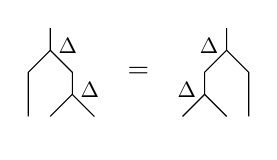
\begin{tikzpicture}[scale=.28]
\node at (0,2){=};
\node at (0,0) {\phantom{$\varepsilon$}};

\draw (2,0)--(3,1)--(3,2)--(4,3)--(4,4);
\draw (4,0)--(3,1);
\draw (4,3)--(5,2)--(5,0);
\node [scale=.8] at (3.2,3.2) {$\Delta$};
\node [scale=.8] at (2.2,1.2) {$\Delta$};

\draw (-2,0)--(-3,1)--(-3,2)--(-4,3)--(-4,4);
\draw (-4,0)--(-3,1);
\draw (-4,3)--(-5,2)--(-5,0);
\node [scale=.8] at (-3.2,3.2) {$\Delta$};
\node [scale=.8] at (-2.2,1.2) {$\Delta$};
\end{tikzpicture}
\end{equation*}
We remark that $U(\A)$-coalgebras in $\Ch$ are precisely coassociative counital coalgebra.

Let $W^{(1)}$ be the chain complex of free $\Z[\S_2]$-modules
\begin{equation*}
\begin{tikzcd}
\Z[\S_2]\{\nu\} &[0pt] \arrow[l, "1-T"'] \Z[\S_2]\{\mu\},
\end{tikzcd} 
\end{equation*}
which is isomorphic to the cellular chains on the standard $\S_2$-equivariant $CW$-structure on the circle
\begin{equation*}
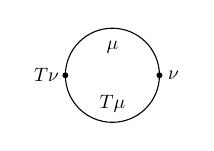
\begin{tikzpicture}[scale=.85]
\draw (0,0) circle (20pt);
\node[scale=.7] at (0,12pt){$\mu$};
\node[scale=.7] at (0,-12pt){$T \mu$};
\node[scale=.7] at (-28pt,0){$T \nu$};
\node[scale=.7] at (26pt,0){$\nu$};
\draw [fill] (-20pt,0) circle [radius=1pt];
\draw [fill] (20pt,0) circle [radius=1pt];
\end{tikzpicture}
\end{equation*}
and let $W^{(0)}$ be the subcomplex generated by $\nu$. We think of $W^{(1)}$ as an $\S_2$-equivariant 1-cell with boundary $W^{(0)}$.

We regard these complexes as $\S$-bimodules concentrated in biarity $(2,1)$, and let $\varphi \colon W^{(0)} \to \A$ be define by sending $T \nu$ and $\nu$ respectively to
\begin{equation*}
	\begin{tikzpicture}[scale=.2]
	\draw (-4,0)--(-4,4);
	\draw (-6,0)--(-6,4);
	\draw [fill] (-6,.2) circle [radius=.2];
	\node [left] at (-6,0) {$\varepsilon$};
	
	\node at (0,.4) {and};
	
	\draw (4,0)--(4,4);
	\draw (6,0)--(6,4);
	\draw [fill] (6,.2) circle [radius=.2];
	\node [right] at (6,0) {$\varepsilon$.};
	\end{tikzpicture}
\end{equation*}
Consider the push-out
\begin{equation*}
\begin{tikzcd}
F(W^{(0)}) \arrow[r, "F(\varphi)"] \arrow[d] & \A \arrow[d, dashed] \\
F(W^{(1)}) \arrow[r, dashed] & \mu \vee_\varphi \A
\end{tikzcd}
\end{equation*}
in the category of props. We think of $\mu \vee_\varphi \A$ as the prop obtained by attaching a $1$-cell in biarity $(2,1)$ to $\A$.

Define $\M$ as the quotient of $\mu \vee_\varphi \A$ by the ideal generated by
\begin{equation*}
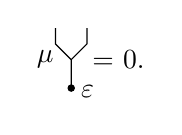
\begin{tikzpicture}[scale=.2]
\draw (5,4)--(5,3)--(6,2)--(6,0);
\draw (7,4)--(7,3)--(6,2);
\node [left] at (5.5,2) {$\mu$};
\draw [fill] (6,.2) circle [radius=.2];
\node [right] at (6,0) {$\varepsilon$};

\node at (9,2) {= 0.};
\end{tikzpicture}
\end{equation*}

We can give a more explicit description of $\M$ using the description of the free prop in terms of $(m,n)$-graphs.
Consider the following elements in $\M$
\begin{equation*}
\counit \in \mathcal M(1,0)_0, \hspace*{.6cm} \coproduct \in \mathcal M(1,2)_0, \hspace*{.6cm} \product \in \mathcal M(2,1)_1,
\end{equation*}
where the decorations by $\varepsilon$, $\Delta$, and $\mu$ are omitted.
Any element in $\M(m,n)$ can be written as a linear combination of the $(m,n)$-graphs generated by these three by grafting, disjoint union and relabeling, modulo the ideals generated by the relations
\begin{equation*}
\qquad \leftcounitality \, , \qquad \rightcounitality \, , \qquad \coassociativity \, , \qquad \productcounit \, .
\end{equation*}
Its chain complex structure is determined using \eqref{e:free prop} by 
\begin{equation*}
\partial\ \counit = 0, \hspace*{.6cm} \partial \ \coproduct = 0, \hspace*{.6cm} \partial \ \product = \ \boundary \, ,
\end{equation*}
and its quasi-isomorphism type is determine by the following result.

\begin{proposition}[\cite{Medina20prop1}]
	The operad $U(\M)$ is an $E_\infty$-operad.
\end{proposition}

We remark that the coassociativity relation is not needed for this result to hold, and that in other contexts it is preferable not to use it since then the associated reduced operad is cofibrant.

